\documentclass[12pt, a4paper, twoside]{report}
\usepackage[T1]{fontenc}
\usepackage{fancyhdr}
\usepackage{graphicx}
\usepackage[unicode,bookmarksnumbered,colorlinks,linktocpage,allcolors=blue]{hyperref}
\usepackage[a4paper,top=40mm,bottom=40mm,inner=40mm,outer=30mm,headheight=15pt,headsep=8mm]{geometry}
\PassOptionsToPackage{defaults=hu-min}{magyar.ldf}
\usepackage[magyar]{babel}
\usepackage{amsthm,mathtools,amssymb}
\usepackage{paralist}
\usepackage{listingsutf8,xcolor}

\DeclareMathOperator{\ctg}{ctg}
\DeclareMathOperator{\tg}{tg}
\theoremstyle{definition}
\newtheorem{definicio}{Definíció}[section]
\theoremstyle{remark}
\pagestyle{fancy}
\fancyhf{}
\fancyhead[EL,OR]{\thepage}
\fancyhead[ER]{\nouppercase{\small\sffamily\leftmark}}
\fancyhead[OL]{\nouppercase{\small\sffamily\rightmark}}
\footnotestyle{rule=fourth}

\lstset{
	inputencoding=utf8/latin2,
	language=Python,
	basicstyle=\footnotesize,
	numbers=left,
	xleftmargin=1cm,
	xrightmargin=1cm,
	breaklines,
	backgroundcolor=\color{gray!30},
	frame=tblr,
	framesep=3pt,
	keywordstyle=\bfseries\color{blue},
	commentstyle=\itshape\color{teal},
}

\title{Assassin's Creed Reneszánsz}
\author{Lovász Ákos\\Programtervező Informatikus}
\date{\today}

\begin{document}
\maketitle
\tableofcontents


\chapter{Ezio Auditore}
\section{Firenze}
Fent, a magasban fáklyák lobogtak, és fénybe borították a Palazzo Vecchio és Bargello tornyait, de valamivel északabbra, a katedrális előtti téren csupán néhány lámpás pislákolt. Ezek némelyike gyengén megvilágította az Arno folyó rakpartját is, ahol a sötétség közeledte még fenyegetőbb volt; az itteni városlakók jónak látták idejekorán nyugovóra  térni  házuk  oltalmában. 

A homályban  már  csak  néhol mozgott  egy-egy  alak:  matrózok,  akik  kapkodva  tekerték  össze  a öteleket, és  súrolták  a  fedélzetet,  miután  befejezték  az  utolsó javításokat hajójuk vitorlázatán, kikötőmunkások, akik sietve hordták a rakományukat a közeli
raktárak biztonságot adó falai közé. Bár az utcák néptelenek voltak, azért az éjszakában ide is jutott némi fény a kocsmák és bordélyházak ablakaiból.

\section{Riválisok}
Immár hét év telt el azóta, hogy Lorenzo de' Medicit választották 
vezetővé Firenzében \emph{Lásd \az{\ref{abra-olasz}}.~képen a Olaszország térképén}, melyet akkoriban vezető nemzetközi bankár- és 
kereskedőcsaládok tettek a világ egyik leggazdagabb városává. Ám a 
családok kegyetlen rivalizálása egyre  nagyobb  feszültséget szült a 
nép körében, és az akkor húszéves fiatalembernek, ha mást nem is, 
legalább a rend és nyugalom látszatát sikerült megteremtenie. 

Ennek ellenére a városban nem szűnt meg a parázsló hangulat, de lángra 
kapott,  valahányszor  az  egyik  tábor  megpróbálta  magához 
kaparintani  a hatalmat - akár azzal, hogy új  szövetségeket kötött, 
akár azzal, hogy megmaradt állhatatos és mozdíthatatlan ellenségnek. 
Firenze  napnyugta  után  nem  volt  biztonságos  az  Úr  1476. 
esztendejében. Még egy jázminillatú, tavaszi estén, amikor az Arno 
folyó bűzét már majdnem elfeledtette a kedvező széljárás, akkor sem 
volt ajánlatos kimerészkedni a szabad ég alá, ha az utcákra leszállt az 
alkony. 

Aznap  a  Hold  magasra  kúszott  fel  az  égen,  hogy  fölényes 
díszszemlét tartson a csillagok miriádnyi serege felett. Fénye ezüstre 
festette  azt  a  nyílt  terecskét  is,  ahol  a  Ponte  Vecchio 
belekapaszkodott a folyó északi partjába. A hídra épült házak boltjai, 
melyeket napközben elárasztott a nyüzsgő tömeg, most sötétek és 
némák voltak. A holdfény egy feketébe öltözött alak körvonalait is 
kirajzolta, aki a Santo Stefano al Ponte templom tetején állt. 

Egy magas és büszke fiatalemberét, aki alig töltötte be tizenhetedik évét. 
Miközben  elmélyülten  vizsgálta  az  alatta  elterülő  teret,  kezét 
szájához  emelte,  és  halk,  de  átható  füttyjelet  hallatott.  Azonnal 
észrevette, hogy válaszul először egy, majd három, aztán egy tucat, 
végül vagy húsz férfi lépett ki a térre a sötét utcákból és az épületek 
boltívei alól. Valamennyien fiatalok voltak, mint ő, övükben kard és 
tőr,  legtöbbjük  feketébe  öltözve,  némelyik  vérvörös,  zöld  vagy 
azúrkék  csuklyát,  kalapot  viselt.  A  vészjósló  külsejű  ifjoncok 
csoportja legyező alakban szétnyílt, mozgásuk kihívóan büszke volt. 

A  fiatalember  lenézett a halvány  fényben úszó, elszánt arcokra, 
melyek  egytől  egyig  rászegeződtek,  és  feje  fölé  emelt  öklével 
konokul tisztelgett nekik. 

— Összetartozunk! -- kiáltotta, miközben a  lentiek  szintén az ég 
felé  lendítették  öklüket.  Többen  közülük  kardjukat  is  kivonták 
hüvelyéből,  megsuhintották  vele  a  levegőt,  és  az  utcakövekről 
egyszerre szállt a magasba lelkes üdvözlésük: - Egységben! 

A fiatalember egy macska ügyességével mászott le a befejezetlen 
homlokzaton a templom oszlopcsarnok alátámasztotta teraszáig. Itt 
szárnyként  kitárta  palástját,  és  egyetlen  ruganyos  szökkenéssel  a 
csoport közepén termett, mely várakozásteljesen gyűlt köré. 

- Csendet, barátaim! - mondta, feltartotta kezét, és ezzel az utolsó 
hang is elnémult. A fiatal férfi komor tekintete fenyegető mosollyá 
változott. 

- Leghűbb társaim, tudjátok-e, miért hívtalak ide benneteket ma 
éjjel?  A  segítségeteket  kérem.  Hosszú  ideje  már,  hogy  családom 
nevét sárba tiporja közös ellenségünk, s a maga szánalmas módján 
igyekszik  lealacsonyítani  bennünket.  Városunk  a  rágalmazásaitól 
hangos, míg én túl sokáig tűrtem hallgatásba burkolózva. Vieri de' 
Pazzi, e név jól ismert előttetek. Egy rühes korcs, ki arra sem volna 
méltó, hogy belerúgjak, most azonban\dots

Ebben  a  pillanatban  lába  előtt  a  földbe  csapódon  egy  jókora 
kődarab, melyet a híd felől hajítottak oda. 

— Elég az ostoba beszédből, grullo!\footnote{hülye}

A szavak ifjú gazdája egyszerre bukkant fel csapatával az említett 
irányból, és ő azonnal tudta, kihez tartozik a hang. Dél felől, a hídon átkelve egy másik társaság közeledett, melyet szintén fiatal férfiak 
alkottak. Vezetőjük láthatóan élvezettel parádézott szerepében, vörös 
köpönyegét pompás csat fogta össze éjfekete bársonygúnyája felett. 
Az ügyes szerkezet kék lapját aranydelfinek és -keresztek díszítették. 
A fiatalember keze rezdületlenül nyugodott kardja markolatgombján. 
Tagadhatatlanul jóképű volt - bár ebből sokat levett a kegyetlen száj 
és  a  gyenge  áll - és,  jóllehet  már  hízásnak  indult,  kétségtelenül 
számolni kellett a karjában és a lábában rejlő erővel. 

— Buona sera, Vieri! Épp rólad beszélgettünk - válaszolt a fiatal 
férfi  kimérten,  és  szándékosan  eltúlzott  udvariassággal  meghajolt, 
miközben tekintete meglepetést színlelt. - De, bocsáss meg a szóért, 
arra  a  legkevésbé  sem  számítottunk,  hogy  személyesen  teszed 
tiszteleted, úgy tudtam, a Pazzik másokat szoktak felbérelni, hogy 
elvégezzék helyettük a piszkos munkát. 

Vieri kihúzta  magát, miután ő és csapata tett még pár  lépést a 
hídon, majd néhány méter után megállt. 

— Ezio  Auditore!  Elkényeztetett  kis  poronty,  még  te  beszélsz? 
Amikor  a  tintanyalók  és  aktakukacok  gyülekezete,  melyet 
családodnak  nevezel,  rohanvást  szalad  a  testőrséghez  védelemért, 
amint  a  veszély  legkisebb  jelét  sejti?  Codardo!\footnote{gyáva}  -  kiáltott,  és 
megragadta kardja  markolatát. - Talán  nem te vagy, aki  fél  saját 
maga kezelésbe venni a dolgokat? 

— Nos,  mit  is  mondhatnék,  Vieri,  ciccione\footnote{dagadék}.  Amikor  utoljára 
találkoztam a húgoddal, Viola igen elégedettnek tűnt a kezeléstől, 
amelyet  tőlem  kapott  -- mondta  Ezio  Auditore,  és  széles  vigyort 
küldött ellensége felé, miközben elégedetten hallgatta társai derült 
kacaját a háta mögül. 

\begin{itemize}
    \item De  tudta, ez alkalommal túl messzire  ment. Vieri arca bíborvörösre változott a dühtől. 
    \begin{enumerate}
        \item - Elég volt, Ezio, te ócska szájhős! Lássuk, a kardodat is olyan jól forgatod-e, mint a nyelved!
        \begin{itemize}
            \item - Öljétek le a fattyúkat! -- üvöltötte.
        \end{itemize}
    \end{enumerate}
\end{itemize}

\Az{\ref{2-fej}}.~fejezetet \az{\pageref{2-fej}}.~oldalon találhatjuk meg.

\section{Az összecsapás}
Ekkor  újabb  kődarab  süvített  át  a  levegőn,  de  ezúttal  nem 
kihívásnak  szánták.  Oldalról  találta  homlokon  Eziót,  akinek 
felszakadt  bőre  alól  vér  buggyant  elő.  Ezio  egy  pillanatra 
hátratántorodott, amint Vieri bandája kőzáport zúdított rá. Emberei is 
épphogy csak magukhoz tértek, mire a Pazzi-banda lefutott a hídról, 
és rárontott Ezióra és csapatára. A támadás olyan gyors volt, hogy 
azonnal közelharccá fajult, mivel még arra is alig lett volna idő, hogy 
kardot  vagy  akár  tőrt  rántsanak,  így  a  két  csoport  eleinte  puszta kézzel ment birokra. 

Az összecsapás vad és brutális volt -- a kőkemény rúgásokat és 
ádáz ökölcsapásokat a repedő csontok hátborzongató hangja kísérte. 
Egy darabig megjósolhatatlan volt a harc kimenetele, aztán Ezio, aki 
a  szemébe  csorgó  vértől  már  alig  látott,  észrevette,  hogy  legjobb emberei közül kettő a földre bukik, és összegörnyed az őket taposó talpak alatt. 

Ekkor közvetlen közelről felhangzott Vieri kacaja, aki 
egy kővel a kezében végzetes csapásra lendítette karját Ezio feje felé. 
Ezio  ösztönösen  elhajolt,  de  hiába  védte  ki  a  széles  ütést,  a 
lendülettől  a  földre  zuhant.  Az  Auditore-tábor  lassan,  de  biztosan kezdett  alulmaradni.  Mielőtt  újra  lábra  állt,  Eziónak  sikerült szabaddá  tennie  tőrét,  és  vaktában  kaszabolva  szerencsésen 
belevágnia egy keménvkötésű Pazzi-orgyilkosba, aki kivont tőrrel és 
karddal készült lemészárolni őt. Ezio tőre a combján érte a támadót, 
átszakítva  a  ruhaszövetet,  az  izmokat  és  az  inakat.  Ellenfeléből 
velőtrázó  üvöltés  szakadt  fel,  eldobta  fegyvereit,  kezét  a  sebére 
szorította,  melyből  bőven  bugyogott  a  vér,  majd  tehetetlenül előrebukott.

Amikor Ezio végül feltápászkodott és körbenézett, azt látta, hogy a 
rivális banda bekerítette valamennyi emberét, és fokozatosan szorítja 
őket a templom fala felé. Érezte, hogy az erő kezd visszatérni lábába, 
és  nekilátott  utat  törni  a  társaihoz.  Egy  nagydarab  Pazzi-legény 
megpróbálta  egy  széles  kardsuhintással  lenyakazni,  de  sikerült 
idejében elkapnia a fejét, és -- ugyanazon lendülettel -- öklével elérnie 
a  robusztus  állkapcsot.  Fogak  repültek  a  levegőben,  és  Ezio 
elégedetten látta, amint az ütéstől letaglózott óriás kábultan zuhan 
térdre.  

Néhány  bátorító  szót  kiáltott  emberei  felé,  pedig 
legszívesebben arra biztatta volna őket, hogy fújjanak visszavonulót, 
amíg  képesek  megőrizni  maradék  méltóságukat.  De  ekkor, 
túlharsogva  a  csata  tomboló  zaját,  egy  zengő,  mégis  kedélyes  és 
nagyon ismerős hang szólította őt a Pazzi- csőcselék mögül. 
— Hé, fratellino1, hát te megint min töröd a fejed? 
Ezio szíve nagyot dobbant a megkönnyebbüléstől, és nagy nehezen 
sikerült kinyögnie néhány fesztelennek tűnő mondatot. 
— Te vagy az, Federico? Már csak te hiányoztál ide! Miért nem 
tudtál ma is kocsmába vagy bordélyba menni, mint rendesen? 
Nem hihetted, hogy kihagyok egy ilyen remek műsort! Tudtam, 
hogy  készülsz  valamire,  így  gondoltam,  ideugrok  és  megnézem, 
hogy a kisöcsém  miként boldogul. De amint  látom,  van  még  mit 
tanulnod! 

Federico Auditore, Ezio pár évvel idősebb bátyja, és az Auditore 
testvérek  közül  a  legidősebb,  nagydarab  fickó  volt,  hatalmas 
étvággyal - italra, szerelemre és bajkeverésre egyaránt éhes. Mielőtt 
még  befejezte  volna  mondókáját,  tüstént  munkához  is  látott. 
Kezdetnek  fogott  két  Pazzi-koponyát,  és  összehasonlító 
töréspróbának  vetette  őket  alá.  

Ezután  --  míg  sietve  átvágott  a tömegen, hogy keblére ölelje öccsét -- csizmája orrával erőteljesen állcsúcson legyintett egy magasabb növésű katonát. Federico lelkét láthatólag  nem  nagyon  viselte  meg  a  körülötte  rendezett  sürgés - forgás. E különös  jelenés  hatására  Ezio  embereibe  visszaszállt  a bátorság,  és  megket tőzött  erővel  harcoltak  tovább.  Az  ellentábor soraiban viszont átmeneti zűrzavar támadt. Ráadásul addigra néhány 
hajógyári  munkás  is  összegyűlt,  hogy  tisztes  távolból  élvezze  az 
előadást,  és  a  Pazzi-fiúk  a  félhomályban  véletlenül  összekevertek 
őket  a  nem  létező  Auditore  felmentő  sereggel.  Ez  a  tény  - 
kiegészítve Federico további mutatványaival (mely mögött Ezio sem 
akart  lemaradni) - az  ellenfél  bősz,  harci  morálját  tökéletes 
pánikhangulattal fűszerezte. 
Az általános felfordulásnak Vieri de' Pazzi dühödt üvöltése vetett véget. 

Visszavonulni! -- kiáltott  emberei  felé,  de  parancsoló  hangja 
elcsuklott  a  kimerültségtől.  Utoljára  még  elkapta  Ezio  pillantását, 
fogai  között  elmorzsolt  egy  néma  szitkot,  majd  eltűnt  a  sötétben.  
Emberei, kik a fáradtságtól járni is alig tudtak, követték vezérüket a 
Ponte  Vecchio  irányába.  Ezio  győztes  szövetségesei  vadul  utánuk 
vetették magukat. 
Ezio is indulni készült velük, de bátyja vaskos keze visszatartotta 
őt. — Egy pillanat -- mondta.

\chapter{Testvéri szeretet}\label{2-fej}
\section{A nyeremény}

\begin{figure}[!ht]
    \centering
    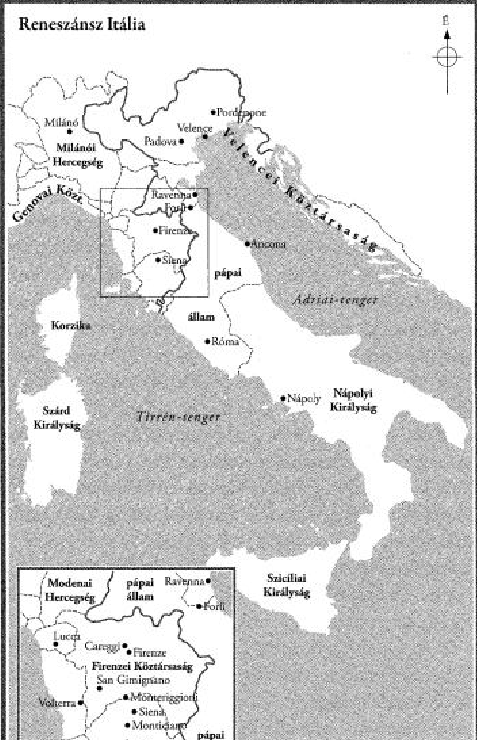
\includegraphics[width=5cm]{italy.png}
    \caption{Olaszország térképe}
    \label{abra-olasz}
\end{figure}

— Ezt hogy érted? Menekülés közben elkapjuk őket! 
— Nyugalom -- mondta Federico egy rosszalló pillantás kíséretében, 
és gyengéden megérintette Ezio felsebzett szemöldökét. 
— Csak egy karcolás. 
— Több ez annál -- döntötte el a kérdést Federico. -- Jobb lesz, ha 
kerítünk neked egy orvost. 

Ezio kiköpött. 
— Nincs  időm  rá,  hogy  orvoshoz  rohangáljak.  Mellesleg\dots  -- 
jegyezte meg bánatosan -- nincs is rá pénzem. 
— Na persze! Gondolom, elpazaroltad nőkre és borra -- vigyorgott 
Federico, és megértően rácsapott testvére vállára. — Pazarlásnak azért nem nevezném. És végül is csak a te példádat követtem. 
Ezio elmosolyodott, de ugyanakkor el is bizonytalanodott. Hirtelen 
tudatosult benne, hogy valóban sajog a feje. 
— Talán  igazad  van,  és  mégsem  ártana  megnézetni.  Gondolom, 
nem tudnál kölcsönadni e célra pár fiorinót\footnote{aranytallért}. 

Federico  megpaskolta  erszényét,  de  az  sehogy  sem  akart 
megcsörrenni. 
— Ami azt  illeti,  jelenleg engem  sem  vet fel a pénz túlzottan -- 
mondta. Ezio elmosolyodott fivére zavarodottságán. 
— Na,  és  te  mire  pazaroltad  el?  Nyilván  adakozásra  és 
bűnbocsánatra. Federico elnevette magát. 
— Jól van, vettem a lapot. 
Körbenézett.  Végeredményben  csak  három  vagy  négy  emberük 
vált harcképtelenné, de már ők is kászálódni kezdtek a csatatéren. 
Felültek, nyögtek egy kicsit, majd elvigyorodtak. Kemény küzdelem volt, de senkinek sem tört csontja. Másrészről viszont sikerült vagy 
fél  tucat  Pazzi-csatlóst  teljesen  kiteríteni,  némelyiküket  csúnyán 
helybenhagyták. 

— Lássuk,  mi  lapul  hőseink  zsebében,  amit  megoszthatnának 
velünk -- javasolta Federico. - Úgy látom, nekik most különben sincs 
szükségük  pénzre.  De  azért  lefogadom,  hogy  azonnal  felélednek, 
amint megpróbálod lehúzni őket. 
— Meglátjuk -- mondta Ezio, azzal nekilátott. Fáradozása nem volt eredménytelen, néhány perc elteltével sikerült összegyűjtenie annyi 
aranyat,  amennyivel  mindkettőjük  erszényét  megtölthette.  

Ezio megcsörgette  az  újonnan  szerzett  vagyont,  és  sokat  sejtetően 
pillantott bátyjára. 
— Elég lesz! -- szólt rá Federico. - Hagyjunk nekik annyit, hogy eljussanak hazáig. Különben is, mi nem volnánk tolvajok, ez csupán hadisarc. A sebed továbbra sem tetszik nekem, irány az orvos. 
Ezio  bólintott,  és  egy  utolsó,  villámgyors  szemlét  tartott  az 
Auditore-győzelem  harcmezején.  Amikor  Federicónak  végleg 
elfogyott a türelme, egyik kezét fivére vállára tette. 
— Gyerünk már! -- mondta, és minden ceremónia nélkül elindult. 
Federico  olyan  sebes  tempót  diktált,  hogy  a  kimerült  

Ezio  alig tudott  lépést  tartani  vele.  Igaz,  amikor  túlságosan  lemaradt  vagy 
rossz  irányt  vett  egy  sikátorban,  bátyja  bevárta  vagy  visszasietett 
érte. 
— Sajnálom,  Ezio,  de  szeretnék  olyan  gyorsan  odaérni  a 
medicóhoz\footnote{orvoshoz}, amilyen gyorsan csak lehet. 

\begin{definicio}\label{definicio}
    1191-ben az orvos általában egy sarlatán volt, aki hamis szerekkel és gyógynövényekkel próbált páciensein segíteni.
 \end{definicio}

\section{A doktor}
Az orvos nem volt messze, ám Ezio percről percre gyengült. Végül 
kikötöttek  egy  félhomályos  helyiségben,  ahol  a  családi  orvosuk 
tartotta praxisát. A sötét tölgyfa asztalokon rézedények és üvegfiolák 
sorakoztak, a falak mentén ismeretlen rendeltetésű eszközök álltak, 
és a plafonról fürtökben lógtak a szárított gyógynövények. Ezio már 
alig állt a lábán. 
\smallskip
Dottore  Ceresa  nem  volt  felhőtlenül  boldog,  hogy  felverték  az 
éjszaka  közepén,  de  amint  egy  gyertyával  közelebb  lépett,  hogy 
megvizsgálja Ezio sebét, azonnal aggodalom fogta el.

— Hmm, fiatalember, ezúttal alaposan helybenhagyta valaki. Jobb 
nem jutott eszébe ma estére, mint összeveretni magát? 
— Becsületbeli  ügyről  volt  szó,  drága  doktor  úr  --  pontosított 
Federico. 
— Az más -- mondta az orvos közömbösen. 
— Katonadolog -- nyögte Ezio félájultan. 
Federico, aki most is szellemeskedés mögé bújtatta aggodalmát, 
még hozzátette: 
Foltozza össze, amennyire lehet! Barátunknak nincs sok fegyvere a 
csinos arcocskáján kívül. 

— Hé,  fottiti\footnote{cseszd meg}!  -- mordult  bátyjára  Ezio  egy  nemzetközileg  ismert 
kézmozdulat kíséretében. 
A doktor rájuk sem  hederített, megmosta kezét, és a  számtalan 
üvegcséi  egyikéből  átlátszó  folyadékot öntött  egy  darab  vászonra. 
Megtisztogatta vele a sebet, amely annyira csípett, hogy Ezio arca 
beletorzult  a  fájdalomba,  majdnem  felpattant  a székről.  Amikor  a 
doktor  úgy  döntött,  hogy  elég  tiszta  a  seb,  fogott  egy  tüt,  és 
birkabelet fűzött át rajta. \emph{\Az{\ref{definicio}}-ban megtalálható magyarázat vélhetőleg erre az egyénre nem vonatkozik.}
— Ez  most  egy  kicsit  jobban  fog  fájni  --  mondta.  Amint  az 
öltésekkel végzett, és bekötözte a sebet, Ezio úgy nézett ki, mint egy 
török, turbánnal a fején az orvos bátorítóan elmosolyodott: 

— Három  fiorino  lesz,  egyelőre.  Pár  nap  múlva  felkeresem  a 
palotájukban, és kiveszem az öltéseket. Az még három fiorino lesz, 
majd akkor. Ronda fejfájása lesz, de túléli. Próbáljon lazítani, úgy 
értem, önmagához képest! És ne aggódjon, a seb nem olyan súlyos, 
mint amilyennek  látszik.  A  jó  hír:  nem  marad  utána sebhely,  így 
ennyivel is kevesebb csalódást okoz majd a hölgyeknek a jövőben. 
Kint, az utcán Federico megölelte öccsét. Előhúzott egy flaskát, és 
Ezio felé nyújtotta. 

— Ne aggódj -- mondta, amikor meglátta Ezio arckifejezését --, ez 
apa  legjobb  gappája\footnote{törkölypálinkája}.  Ilyen  állapotban  az  anyatejnek  sem  vennéd 
nagyobb hasznát. 
Mindketten ittak, és érezték, ahogy a tüzes folyadék felmelegíti 
őket.\cite{BERNE}

De  hol  lehetett  Federico?  Felkapaszkodott  a torony  tövéhez,  és 
visszafordult, hogy megnézze, merről jött. Épp időben nézett hátra, 
hogy lássa, amint a bátyja átvitorlázik a levegőn. Federico stabilan 
érkezett, de a súlya alatt kibillent a helyéről pár vörös agyagcserép, 
és kis híján kicsúszott alóla a lába is, ahogy a cserepek elsurrantak a 
tetőn,  átbuktak  a  peremen,  és  pár  másodperccel  később  hangos 
csattanással zúzódtak szét az utcakövön. De Federico már vissza is 
nyerte  az  egyensúlyát,  és  zihálva,  de  széles,  büszke  mosollyal  az 
arcán egyenesedett fel.

,,Szeretem a sört, de a matematikai képleteket mégjobban'' - Lovász Ákos, 2021
\smallskip

\begin{equation} \label{keplet}
    \emph{g}\ \colon\mathbb{R}\ \setminus
    \left\{n\pi \colon n \in\mathbb{Z}\right\}\to\mathbb{R},\quad
    \emph{g}(\emph{x}):=
    \begin{cases}
        \frac{\ctg^3(\emph{x})\sin(\emph{2x})}{\emph{x}-1},&\text{ha }\emph{x} > 1,\\
        \emph{x}(\frac{\emph{x}^2}2)+1,&\text{különben}.
    \end{cases}
    \end{equation}\cite[A képlet forrása]{TomacsTibor}
    \Az{\eqref{keplet}} egyenlet segítségével oldhatjuk meg a feladatot.

\lstinputlisting{forraskod.py}

\begin{thebibliography}{4}
    \bibitem{BERNE}\textsc{Anton Gill}: \emph{Assassin's Creed Reneszánsz}, November 11, 2009, 	Penguin Books.
    \bibitem{OLIVER}\textsc{Oliver Bowden}: \emph{A mese bűvölete és a bontakozó gyermeki lélek}, Budapest, 1985, Gondolat Kiadó.
    \bibitem{EKE} Dr.Kovásznai Gergely -Számítás elmélet Diasor.
	\bibitem{TomacsTibor} Dr. Tómács Tibor Beadandó LATEX-feladatok
\end{thebibliography}

\end{document}